\section{Graphs}

A graph is a visual representation of a relation. For a function
\[
y=f(x),
\]
we usually place \(x\) on the horizontal axis and \(y\) on the vertical axis. Each point on the graph has coordinates
\[
(x,f(x)).
\]

\begin{center}
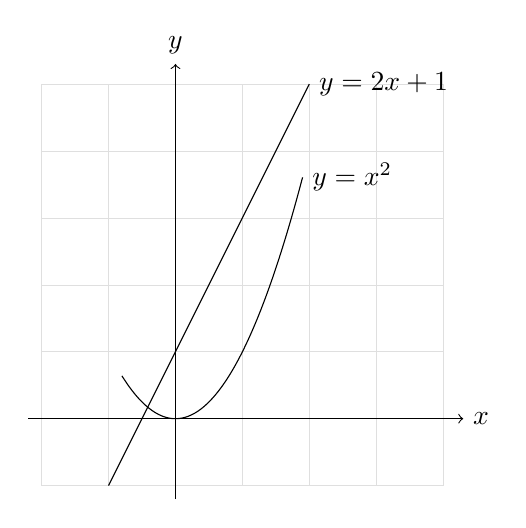
\begin{tikzpicture}[scale=0.85]
    \draw[step=1, gray!25, very thin] (-2,-1) grid (4,5);
    \draw[->] (-2.2,0) -- (4.3,0) node[right] {$x$};
    \draw[->] (0,-1.2) -- (0,5.3) node[above] {$y$};
    \draw[domain=-0.8:1.9, smooth, samples=80] plot (\x,{\x*\x});
    \draw[domain=-1.0:2.0, smooth, samples=2] plot (\x,{2*\x+1});
    \node[right] at (1.9,3.61) {$y=x^2$};
    \node[right] at (2.0,5.0) {$y=2x+1$};
\end{tikzpicture}
\end{center}

A graph is not only a picture. It contains information.

\begin{center}
\begin{tabular}{@{}ll@{}}
\toprule
What to look for & What it tells us \\
\midrule
Increasing or decreasing parts & how the output changes \\
Steep or flat parts & whether change is rapid or slow \\
Zeros & where the function takes value \(0\) \\
Maximum or minimum values & where the output is largest or smallest locally \\
Shape & whether the relation is linear or nonlinear \\
\bottomrule
\end{tabular}
\end{center}

For example, the graph of \(f(x)=2x+1\) is a straight line. The graph of \(f(x)=x^2\) is a parabola.

\begin{summarybox}
A formula gives a symbolic description. A graph gives a visual description. They are two ways of representing the same relation.
\end{summarybox}
